\documentclass[12pt, a4paper]{article}
\usepackage[utf8]{inputenc}
\usepackage{mathtools}
\usepackage{amsthm}
\usepackage{cancel}
\usepackage{graphicx}
\graphicspath{ {../images/} }

\usepackage{listings}
\usepackage{xcolor}

\usepackage[T1]{fontenc}

\definecolor{codegreen}{rgb}{0,0.6,0}
\definecolor{codegray}{rgb}{0.5,0.5,0.5}
\definecolor{codepurple}{rgb}{0.58,0,0.82}
\definecolor{backcolour}{rgb}{0.95,0.95,0.92}

\lstdefinestyle{mystyle}{
    backgroundcolor=\color{backcolour},   
    commentstyle=\color{codegreen},
    keywordstyle=\color{blue},
    numberstyle=\tiny\color{codegray},
    stringstyle=\color{codegreen},
    basicstyle=\ttfamily\footnotesize,
    breakatwhitespace=false,         
    breaklines=true,                 
    captionpos=b,                    
    keepspaces=true,                 
    numbers=left,                    
    numbersep=5pt,                  
    showspaces=false,                
    showstringspaces=false,
    showtabs=false,                  
    tabsize=2
}

\lstset{style=mystyle}

\title{Obligatorisk oppgave 1, MAT1110, Vår 2021}
\author{Cory Alexander Balaton}
\date{}

\begin{document}

\maketitle 
\newpage

\section*{Oppgave 1}

a) 

\begin{equation}
    \textbf{r}(t) = \left(a \cdot arcsinh\left(\frac{t}{a}\right), \sqrt{t^2 + a^2}\right)
\end{equation}

\begin{equation}
    \textbf{r}'(t) = \left(\frac{1}{\sqrt{1 + (\frac{t}{a})^2}}, \frac{t}{\sqrt{t^2 + a^2}}\right)
\end{equation}

\begin{equation}
    \begin{split}
        ||\textbf{r}'(t)|| &= \sqrt{\left(\frac{1}{\sqrt{1 + (\frac{t}{a})^2}}\right)^2 + \left(\frac{t}{\sqrt{t^2 + a^2}}\right)^2} \\
                           &= \sqrt{\frac{1}{1 + \frac{t^2}{a^2}} + \frac{t^2}{t^2 + a^2}} \\
                           &= \sqrt{\frac{a^2}{a^2 + t^2} + \frac{t^2}{t^2 + a^2}} \\
                           &= \sqrt{\frac{a^2 + t^2}{a^2 + t^2}} \\
                           &= \sqrt{1} \\
                           &= \underline{\underline{1}}
    \end{split}
\end{equation}

b) For å vise at buelengden blir $2b$, så må man ta $\int_{-b}^b ||\textbf{r}'(t)|| dt$

\begin{equation}
    \begin{split}
        l &= \int_{-b}^b ||\textbf{r}'(t)|| dt \\
          &= \int_{-b}^b 1 dt \\
          &= [t + C]_{-b}^b \\
          &= b - (-b) \\
          &= \underline{\underline{2b}}
    \end{split}
\end{equation}

\newpage

c) Vi kan bruke det faktumet at $tan \theta = \frac{S \cdot sin \theta}{S \cdot cos \theta}$ og gjøre noen substitusjoner til å få:

\begin{equation}
    \begin{split}
        Tan \theta &= \frac{S \cdot sin \theta}{S \cdot cos \theta} \\
                   &= \frac{\frac{S_0 \cdot s}{a}}{S_0} \\
                   &= \underline{\underline{\frac{s}{a}}}
    \end{split}
\end{equation}

Siden $tan \theta = \frac{dy}{dx} = \frac{\frac{dy}{dt}}{\frac{dx}{dt}}$, så kan man lage likningen:

\begin{equation}
    \begin{split}
        \frac{dy}{dx} &= \frac{\frac{t}{\sqrt{t^2 + a^2}}}{\frac{1}{\sqrt{1+\frac{t^2}{a^2}}}} \\
                      &= \frac{\frac{t}{\sqrt{t^2 + a^2}}}{\frac{a}{\sqrt{t^2 + a^2}}} \\
                      &= \underline{\underline{\frac{t}{a}}}
    \end{split}
\end{equation}

deretter setter man svaret fra likning 5 lik svaret fra likning 6 og får:

\begin{equation}
    \begin{split}
        \frac{s}{a} &= \frac{t}{a} \\
                  s &= t 
    \end{split}
\end{equation}

\newpage

d)
\lstinputlisting[language=Python]{../Python/1d.py}

Programmet over produserer grafen under:

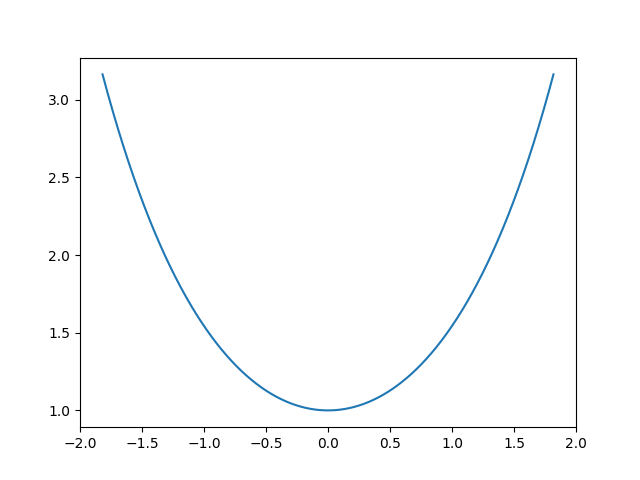
\includegraphics[scale=0.8]{1d}

\newpage

\section*{Oppgave 2}

a) For at to vektorfelt skal stå normalt på hverandre, så må prikkproduktet av dem være lik 0. 
Derfor kan man lett sjekke om $\textbf{F}$ står normalt på $\textbf{F}^\perp$:

\begin{equation}
    \begin{split}
        \textbf{F} \cdot \textbf{F}^\perp &= (ax + by, cx + dy) \cdot (-cx -dy, ax + by) \\
                                          &= -(ax + by)(cx + dy) + (ax + by)(cx + dy) \\
                                          &= \underline{\underline{0}}
    \end{split}
\end{equation}

b) For at $\textbf{F}^\perp$ skal være et konservativt felt, så må $\frac{\partial \textbf{F}^\perp_2}{\partial x} = \frac{\partial \textbf{F}^\perp_1}{\partial y}$.

\begin{equation}
    \begin{split}
        \frac{\partial \textbf{F}^\perp_2}{\partial x} &= \frac{\partial \textbf{F}^\perp_1}{\partial y} \\
                    \frac{\partial}{\partial x} ax +by &= \frac{\partial}{\partial x} -cx -dy \\
                                                     a &= -d \\
                                                     d &= -a
    \end{split}
\end{equation}

For at $\textbf{F}^\perp$ skal være konservativt, så må $\underline{\underline{d = -a}}$

c) Vi har likningen $\phi(\textbf{r}(t)) = K$ der $\textbf{r}(t)$ er en kurve på nivåkurven K, og $\textbf{r}'(t)$ tangerer på ethvert punkt på
$\textbf{r}(t)$. Vi kan dermed bruke kjerneregelen på $\phi(\textbf{r}(t)) = K$, og man får:

\begin{equation}
    \begin{split}
        \frac{d}{dt}\phi(\textbf{r}(t)) &= \frac{d}{dt} K \\
        \nabla\phi(\textbf{r}(t)) \cdot \textbf{r}'(t) &= 0
    \end{split}
\end{equation}

Siden $\textbf{r}'(t)$ tangerer nivåkurven overalt, og prikkproduktet er lik $0$, så må $\nabla\phi(\textbf{r}(t))$ være normal på nivåkurven.

d) Hvis $\nabla\phi(x,y) = k \cdot \textbf{F}^\perp(x,y)$, så betyr det at de er parallelle, og siden $\textbf{F}(x,y)$ står normalt på $\textbf{F}^\perp(x,y)$,
så vil $\textbf{F}$ også være normal på $\nabla\phi(x,y)$, som betyr at $\textbf{F}(x,y)$ vil være parallell med nivåkurvene.

\begin{equation}
    \begin{split}
        \textbf{F}^\perp(x,y) = (-cx + ay, ax + by)
    \end{split}
\end{equation}

\begin{equation}
    \begin{split}
        \phi(x,y) &= cx^2 - 2axy - by^2 \\
        \nabla\phi(x,y) &= (2cx - 2ay, -2by - 2ax) \\
        \nabla\phi(x,y) &= -2(-cx + ay, ax + by) \\
        \nabla\phi(x,y) &= -2 \cdot \textbf{F}^\perp(x,y) \\
    \end{split}
\end{equation}

siden vi har vist at $\nabla\phi(x,y) || \textbf{F}^\perp(x,y)$, så vil $\textbf{F}$ være parallell med nivåkurvene. 

e) For å avgjøre hva for slags nivåkurver vi får ved ulike verdier av a, b, og c, så må vi ta determinanten av den kvadratiske matrisen 
$
\begin{bmatrix}
    c  & -a \\
    -a & -b \\
\end{bmatrix}
$.

\begin{equation}
    \begin{split}
        det \begin{vmatrix}
            c  & -a \\
            -a & -b \\
        \end{vmatrix} = -cb - a^2 = -(cb + a^2)
    \end{split}
\end{equation}

Dette betyr at hvis $-(cb + a^2) < 0 \Rightarrow cb + a^2 > 0$ så er nivåkurvene hyperbler, og hvis $-(cb + a^2) > 0 \Rightarrow cb + a^2 < 0$, så er kurvene ellipser.

\newpage

f) Ved å skrive et lite program:
\lstinputlisting[language=Python]{../Python/2f.py}

får vi ut to grafer: \\
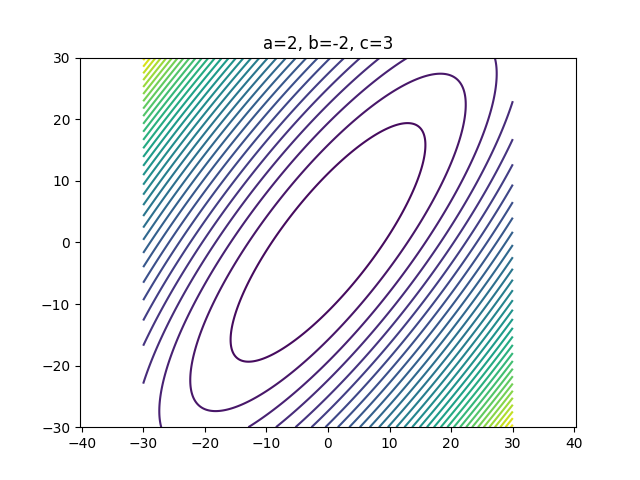
\includegraphics[scale=0.5]{ellipse}
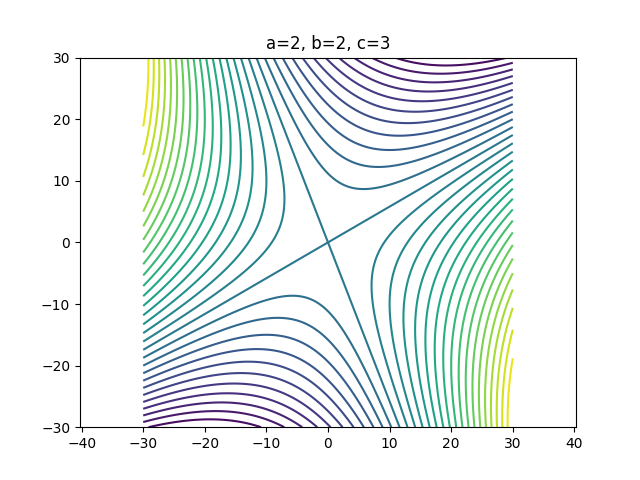
\includegraphics[scale=0.5]{hyperbolic}



    
\end{document}